\section{Хеши и хеш-таблицы}

Пусть есть пространство ключей $U$ и семейство хэш-функций $H : U \to [m]$. $H$ называется универсальным семейством хэш-функций для $U$, если $\forall x, y \in U : |\{h \in H : h(x) = h(y)\}| \leq \frac{|H|}{m}$. Семейство хэш-функций называется $k$-независимым, если $\forall (x_1, \dots, x_k) \in U^k$ ($x_i \neq x_j$), $\forall (y_1, \dots, y_k) \in [m]^k : P[h(x_1) = y_1 \land \dots \land h(x_k) = y_k] = m^{-k}$

При открытой адресации всё хранится в одном массиве, разрешение коллизий происходит следующим образом - выбирается правило, по которому изменяется значение хеша, пока бакет с соответствующим хешем занят. Например, можно прибавлять 1 со взятием по модулю размера хеш-таблицы. В закрытой адресации поступаем по другому - в каждом бакете храним какую-то структуру (например, односвязный список), в которой будут храниться ключи с одинаковым хешем и по которой будем осуществлять поиск/вставку при запросе к данному ключу.

Фильтр Блума - храним битсет длины $m$, выбираем $k$ хеш функций (которые должны быть независимыми в совокупности), для элемента $x$ ставим единички в биты $h_1(x), \ h_2(x), \dots, \ h_k(x)$. Вероятность того, что какой-то бит останется нулевым после добавления $n$ элементов, равна $(1 - \frac{1}{m})^{kn} \approx e^{-\frac{kn}{m}}$. Ложноположительное срабатывание - все биты, принадлежащие хешу какого-то ключа, оказываются единичными, вероятность равна $(1 - e^{-\frac{kn}{m}})^k$

Двухуровневая схема идеального хеширования: выбирается случайная функция $U \to [N]$, заменяется до тех пор, пока $\sum |B_i|^2 > 2N$ (где $B_i$ - бакет $i$), после чего для бакета $i$ выделяем $|B_i|^2$ ячеек и находим функцию $h_i$, которая является идеальной. Пруфы ниже (на английском):

\centering 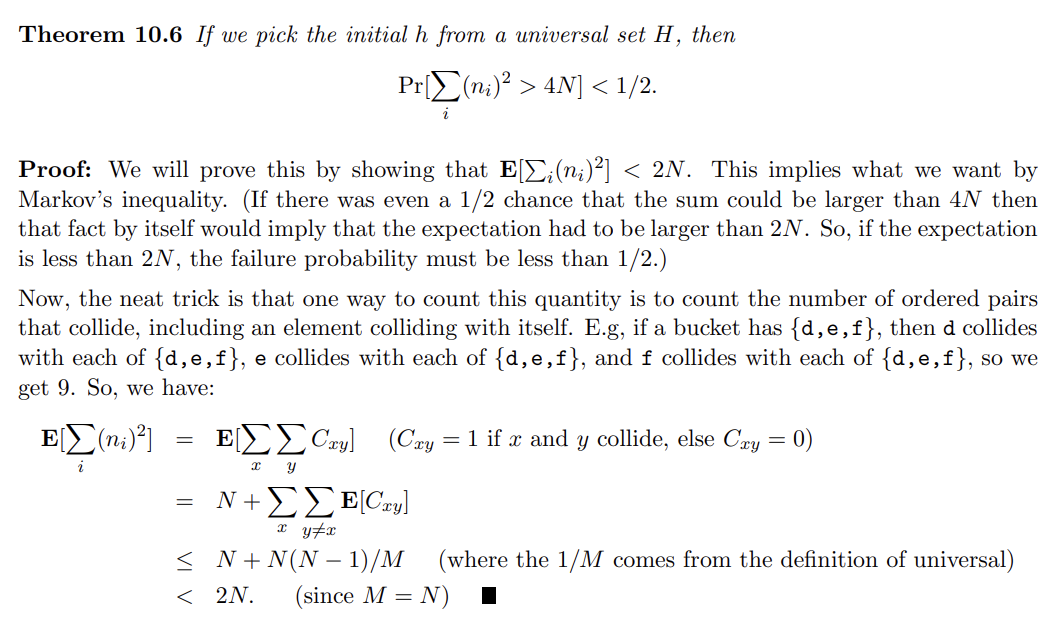
\includegraphics[scale=0.35]{static/perfect_hash_l1.png}

\centering 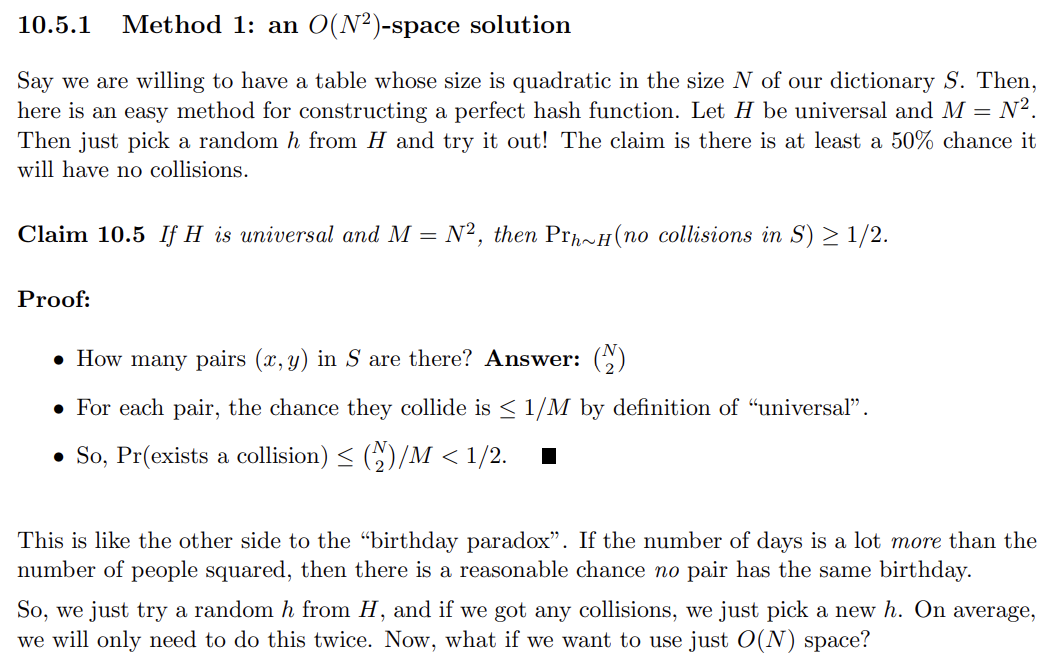
\includegraphics[scale=0.35]{static/perfect_hash_l2.png}
